\documentclass{article}
\usepackage[italian]{babel}
\usepackage[utf8]{inputenc}
\usepackage[margin=75pt]{geometry}
\usepackage{amsmath}
\usepackage{graphicx}
\usepackage{spverbatim}
\usepackage{hyperref}

%IMPORT CODE
%\usepackage{minted}
\usepackage{listings}
\usepackage{color}

\definecolor{dkgreen}{rgb}{0,0.6,0}
\definecolor{gray}{rgb}{0.5,0.5,0.5}
\definecolor{mauve}{rgb}{0.58,0,0.82}

\lstset{frame=tb,
	language=Haskell,
	aboveskip=3mm,
	belowskip=3mm,
	showstringspaces=false,
	columns=flexible,
	basicstyle={\small\ttfamily},
	numbers=none,
	numberstyle=\tiny\color{gray},
	keywordstyle=\color{blue},
	commentstyle=\color{dkgreen},
	stringstyle=\color{mauve},
	breaklines=true,
	breakatwhitespace=true,
	tabsize=3
}

% in way to comment a block
\long\def\/*#1*/{}

\title{\textbf{Relazione sul Progetto d'Esame}}
\author{Francesco Rombaldoni}
\date{\small Università degli Studi di Urbino Carlo Bo\\
	Insegnamento di Programmazione Logica e Funzionale}

\begin{document}
	\maketitle
	
%	Prepared for a formal document
%	\newpage
	
	%\tableofcontents
	%\newpage

\section{Specifica del Problema}
Scrivere un programma Haskell e un programma Prolog che, dato l'inserimento di due rilevamenti satellitari in formato di coordinata unica nella quale la latitudine e la longitudine sono rappresentate in formato D.M.G internazionale, effettuano le seguenti operazioni: controllo della validità dei rilevamenti inseriti dall'utente, calcolare e riportare (sempre in formato di coordinata unica) per ogni rilevamento la corrispettiva latitudine e longitudine in formato decimale, calcolare e riportare la distanza in chilometri compresa tra i due rilevamenti satellitari, calcolare e riportare l'angolo di rotta espresso in gradi (sia diretto che inverso) che unisce i due rilevamenti inseriti.
\newline
\newline
%\emph{[Confrontare lo svolgimento delle fasi successive con quanto riportato nelle prossime pagine.]}\\
\newpage
			
\section{Analisi del Problema}
\subsection{Dati di Ingresso del Problema}
Per ciascuna delle quattro operazioni, i dati d'ingresso del problema sono rappresentati da due rilevamenti satellitari in formato di coordinata unica nella quale la latitudine e la longitudine sono rappresentate in formato D.M.G internazionale. \\
Esempio di rilevamento accettato: N 40 45 36.000 - E 73 59 2.400.

\subsection{Dati di Uscita del Problema}
Per ogni inserimento di una coppia di rilevamenti nel formato prima specificato i dati d' uscita del problema, rispettivamente alle ultime tre operazioni descritte all'interno della sezione di specifica del problema, sono: il risultato della conversione delle coordinate del primo rilevamento inserito dal formato D.M.G internazionale a quello decimale, il risultato della conversione delle coordinate del secondo rilevamento inserito dal formato D.M.G internazionale a quello decimale, il risultato del calcolo della distanza compresa tra i due rilevamenti inseriti, il risultato del calcolo dell'angolo di rotta diretto che unisce i due rilevamenti, il risultato del calcolo dell'angolo di rotta inverso che unisce i due rilevamenti. 
L'operazione di controllo della validità dei rilevamenti immessi restituisce un messaggio d'errore nel caso in cui i rilevamenti inseriti non risultino validi. Il messaggio d'errore è composto da due parti, dove nella prima parte viene descritto il tipo d'errore commesso, nella seconda viene riportata la porzione di coordinata nella quale è stato rilevato l'errore. 

\subsection{Relazioni Intercorrenti tra i Dati del Problema}
Dato l'inserimento di due rilevamenti nel formato prima specificato, le operazioni in questione sono definite come segue:
\begin{itemize}
	\item Controllo della validità dei rilevamenti; per ogni rilevamento inserito, si verifica che la sua lunghezza sia di trentuno caratteri (considerando anche gli spazi), altrimenti viene restituito un messaggio d'errore. Successivamente si verifica se la latitudine e la longitudine siano corrette, in particolare si verifica se il "segno" della latitudine sia "N" oppure "S", in caso contrario viene restituito un messaggio d'errore, la stessa cosa vale pure per la longitudine, controllando che il "segno" sia "E" oppure "W". Il "corpo" della latitudine e della longitudine si verifica nello stesso modo, controllando se i "gradi" siano compresi tra il valore zero e il valore ottantanove (estremi compresi) e se i "primi" ed i "secondi" siano compresi tra il valore zero ed il valore cinquantanove, qualora i valori dei "gradi", dei "primi" o dei "secondi" dovessero risultare sbagliati, verrà restituito un messaggio d'errore relativo al valore rilevato come errato.
	
	\item Conversione delle coordinate dalla forma D.M.G internazionale alla forma decimale; data una qualsiasi coordinata il passaggio dalla forma D.M.G internazionale alla forma decimale è definito come segue: \\
	Decimali = (Gradi + ( ((Secondi / 60) + Primi) / 60 ) * (-1) se il Segno è  S o W).
	
	\item Calcolo della distanza compresa tra i due rilevamenti inseriti;  data una coppia di rilevamenti rispettivamente denominati "A" e "B" la distanza compresa è definita come: \\
	$Distanza(A, B) = R * \arccos(\sin(latA * \pi / 180) * \sin(latB * \pi / 180) + \cos(latA * \pi / 180) * \cos(latB * \pi / 180) * \cos((lonA - lonB) * \pi / 180)). $\\
	dove R rappresenta il raggio della Terra.
	
	\item Calcolo dell'angolo di rotta diretto e inverso tra i due rilevamenti inseriti; data una coppia di rilevamenti rispettivamente denominati "A" e "B" e data la condizione che la latitudine e la longitudine siano diverse l'angolo di rotta diretto e inverso compresa è definita come: \\
	$\Delta\Phi = \ln( \tan(latB * \pi / 360 + \pi / 4 ) / \tan(latA * \pi / 360 + \pi / 4 )). $\\
	$ \Delta Lon = abs(lonA - lonB). $ \\
	$ Angolo Diretto = atan2((\Delta Lon * \pi / 180), (abs(\Delta\Phi))) / \pi * 180.$\\
	$ Angolo Inverso = Angolo Diretto+ 180.$\\
	Nel caso in cui la latitudini dei due rilevamenti siano identiche:\\
	$\Delta\Phi = \pi / 180 * 0.000000001.$\\
	Nel caso in cui la longitudini dei due rilevamenti siano identiche:\\
	$\Delta Lon = \pi / 180 * 0.000000001.$\\
\end{itemize}
\newpage

\section{Progettazione dell'Algoritmo}
\subsection{Scelte di Progetto}
Il rilevamento immesso dall'utente (nel quale è presente una coppia di coordinate), viene catturato dal terminale sotto forma di "stringa", pertanto il rilevamento è gestibile come una lista di caratteri "char". Per estrarre le coordinate vengono effettuate delle operazioni arbitrarie volte ad isolare le varie parti della lista d'interesse, proprio perchè queste operazioni sono arbitrarie e non vincolate da un simbolo presente nella lista, si controlla che quest'ultima sia precisamente di trentuno caratteri considerando anche gli spazi.\\
Per scelta architetturale si è pensato d'implementare una sola funzione/predicato per la conversione delle coordinate dal formato D.M.G internazionale al formato decimale, questo comporta che le coordinate sono gestite in coppia (ovvero quando la latitudine e la longitudine sono riunite per formare un rilevamento) solo in due momenti chiave, cioè quando la latitudine e la longitudine vengono estratte dal rilevamento inserito dall'utente per venire poi gestite separatamente (quindi non più in coppia) e quando la latitudine e la longitudine, dopo essere state convertite dal formato D.M.G internazionale al formato decimale, vengono riunite per formare quindi un rilevamento in formato decimale.\\
 Un'ulteriore decisione architetturale è stata presa nella gestione delle singole coordinate, infatti la latitudine e la longitudine individuate all'interno della lista di caratteri "char" vengono convertite rispettivamente in due "tuple" distinte definite come segue: (Char, Integer, Integer, Float) ovvero (Segno, Gradi, Primi, Secondi), in modo da poter semplificare l'implementazione delle funzioni/predicati atti alla conversione delle coordinate dal formato D.M.G internazionale al formato decimale. Nel caso specifico del Prolog al posto delle "tuple" vengono utilizzate delle liste contenenti tipi di dato diversi definite come segue: [Char, Integer, Integer, Float] ovvero [Segno, Gradi, Primi, Secondi].
 
\subsection{Passi dell'Algoritmo}
I passi dell'algoritmo sono diversi a seconda del tipo d'operazione:
\begin{itemize}
	
	\item Controllo della validità dei rilevamenti:
	\begin{enumerate}
		\item La "stringa" contenente il rilevamento inserito dall'utente viene convertita in una lista di caratteri "char".
		\item Viene valutato se la lista così ottenuta sia di dimensione trentuno, in caso contrario viene restituito un messaggio d'errore.
		\item La lista viene manipolata per isolare le informazioni relative alla latitudine da inserire nella "tupla"/lista che rappresenta la latitudine in formato D.M.G internazionale.
		\item Si esegue la verifica delle informazioni contenute all'interno della "tupla"/lista rappresentante la latitudine in formato D.M.G internazionale, verificando nel seguente ordine:  la correttezza del "segno" controllando che sia "N" oppure "S", i "gradi" controllando che siano compresi tra il valore zero ed il valore ottantanove (estremi compresi), i "primi" ed i "secondi" controllando che entrambi i valori siano compresi tra il valore zero ed il valore cinquantanove (estremi compresi). Nel caso in cui uno dei quattro controlli dovesse rilevare un errore, viene restituito un messaggio nel quale si descrive il tipo d'errore riscontrato.
		\item La lista iniziale viene nuovamente manipolata per isolare le informazioni relative alla longitudine da inserire nella "tupla"/lista che rappresenta la longitudine in formato D.M.G internazionale.
		\item Si esegue la verifica delle informazioni contenute all'interno della "tupla"/lista rappresentante la longitudine in formato D.M.G internazionale, verificando nel seguente ordine:  la correttezza del "segno" controllando che sia "E" oppure "W", i "gradi" controllando che siano compresi tra il valore zero ed il valore centosettantanove (estremi compresi), i "primi" ed i "secondi" controllando che entrambi i valori siano compresi tra il valore zero ed il valore cinquantanove (estremi compresi). Nel caso in cui uno dei quattro controlli dovesse rilevare un errore, viene restituito un messaggio nel quale si descrive il tipo d'errore riscontrato.
	\end{enumerate}

	\item Conversione delle coordinate dalla forma D.M.G internazionale alla forma decimale:
	\begin{enumerate}
		\item La "tupla"/lista contenente la latitudine in formato D.M.G internazionale viene convertita in formato decimale applicando la seguente formula: \\Decimali = (Gradi + ( ((Secondi / 60) + Primi) / 60 ) * (-1) se il Segno è  S ). 
		\item La "tupla"/lista contenente la longitudine in formato D.M.G internazionale viene convertita in formato decimale applicando la seguente formula: \\Decimali = (Gradi + ( ((Secondi / 60) + Primi) / 60 ) * (-1) se il Segno è  W ).
		\item Le coordinate così ottenute vengono riunite all'interno di una "tupla"/lista così definita: (latitudine decimale, longitudine decimale)/[latitudine decimale, longitudine decimale].
	\end{enumerate}

	\item Calcolo della distanza compresa tra i due rilevamenti inseriti: 
	\begin{enumerate}
		\item Data una coppia di rilevamenti in formato decimale rispettivamente denominati "A" e "B", il calcolo della distanza compresa tra i due rilevamenti viene calcolata applicando la seguente formula: \\$Distanza(A, B) = R * \arccos(\sin(latA * \pi / 180) * \sin(latB * \pi / 180) + \cos(latA * \pi / 180) * \cos(latB * \pi / 180) * \cos((lonA - lonB) * \pi / 180)). $
	\end{enumerate}

	\item  Calcolo dell'angolo di rotta diretto e inverso tra i due rilevamenti inseriti:
	\begin{enumerate}
		\item  Si considera una coppia di rilevamenti in formato decimale rispettivamente denominati "A" e "B".
		\item Si calcola il $\Delta\Phi$ dei rilevamenti nel caso in cui le latitudini dei suddetti siano diverse applicando la seguente formula:\\ $\Delta\Phi = \ln( \tan(latB * \pi / 360 + \pi / 4 ) / \tan(latA * \pi / 360 + \pi / 4 )). $\\
		Nel caso in cui le latitudini dei due rilevamenti siano identiche, il $\Delta\Phi$ viene calcolato in questo modo:\\ $\Delta\Phi = \pi / 180 * 0.000000001.$
		\item Si calcola il $\Delta Lon$ dei rilevamenti nel caso in cui le latitudini dei suddetti siano diverse applicando la seguente formula:\\ $ \Delta Lon = abs(lonA - lonB). $\\
		Nel caso in cui le latitudini dei due rilevamenti siano identiche, il $\Delta Lon$ viene calcolato in questo modo:\\ $\Delta Lon = \pi / 180 * 0.000000001.$
		\item Si calcola quindi l'angolo di rotta diretto tra i due rilevamenti applicando la seguente formula:\\ $ Angolo Diretto = atan2((\Delta Lon * \pi / 180), (abs(\Delta\Phi))) / \pi * 180.$\\
		\item L'angolo di rotta inverso tra i due rilevamenti è calcolato applicando la seguente formula: \\ $ Angolo Inverso = Angolo Diretto+ 180.$\\
	\end{enumerate}

\end{itemize}
\newpage

\section{Implementazione dell'Algoritmo}
\raggedright
\underline{File sorgente \textbf{Detection.hs:}}
\lstset{language=Haskell}
\begin{lstlisting}
module Detection where
import GHC.Float
import GHC.Num

{-**** Defining the Functions to Work with Detections. ****-}
            
{-Get the Longitude string part from the Detection string.
* Input: A Detection String.
* Output: A String without the Latitude string part.-}
split :: String -> String
split = drop 17 

{-Verify if the Detection string Has the Right Lenght.
* Input: A Detection String.
* Output: A Boolean that is 1 If the Detection string Has the Right Lenght, 0 Otherwise.-}
verifyLenght :: String -> Bool
verifyLenght [] = error "Null Argument"
verifyLenght st
               | length st < 32 || length st > 32 = False
               | otherwise = True

{-Verify if the Detection string is in the Right Format.
* Input: A Detection String.
* Output: A Boolean that is 1 If the Detection string is in the Right Format, 0 Otherwise.-}
verifyFormat :: String -> Bool
verifyFormat [] = error "Null Argument"
verifyFormat st
               | not (verifyLenght st) = False
               | st !! 1 /= ' ' = False
               | st !! 4 /= ' ' = False
               | st !! 7 /= ' ' = False
               | st !! 14 /= ' ' = False
               | st !! 16 /= ' ' = False
               | st !! 18 /= ' ' = False
               | st !! 22 /= ' ' = False
               | st !! 25 /= ' ' = False
               | otherwise = True

{-Get the Latitude Tupla from the Detection string.
* Input: A Detection String.
* Output: A Tupla Containing the Latitude in D.M.G format,
   (Sign, Degrees, Primes, Latters).-}
getLatitude :: String -> (Char, Int, Int, Float)
getLatitude [] = error "Null Argument"
getLatitude st
              | not (verifyFormat st) = error ("Invalid Argument: " ++ st)
              | otherwise = (head st, read (take 2 (drop 2 st)) :: Int, read (drop 5 (take 7 st)) :: Int, read (drop 8 (take 14 st)) :: Float)

{-Get the Longitude Tupla from the Detection string.
* Input: A Detection String.
* Output: A Tupla Containing the Longitude in D.M.G format,
   (Sign, Degrees, Primes, Latters).-}
getLongitude :: String -> (Char, Int, Int, Float)
getLongitude [] = error "Null Argument"
getLongitude st
               | not (verifyFormat st) = error ("Invalid Argument: " ++ st)
               | otherwise = (head (split st), read (take 3 (drop 2 (split st))) :: Int, read (drop 6 (take 8 (split st))) :: Int, read (drop 9 (take 15 (split st))) :: Float)

{-** Verify if Latitude & Longitude are Real. **-}

{-Verify if the Latitude Degrees are Real.
 * Input: A Latitude Tupla.
 * Output: True if the Latitude Degrees are Real. False otherwise.-}
verifyLatDeg :: (Char, Int, Int, Float) -> Bool 
verifyLatDeg (s, x, y, z)
                         | x < 0 || x > 89 = error ("Wrong Degree in: " ++ pt)
                         | otherwise = True
                         where
                              pt = " " ++ show s ++ " " ++ show x ++ " " ++ show y++ " " ++ show z

{-Verify if the Longitude Degrees are Real.
 * Input: A Longitude Tupla.
 * Output: A Boolean that is True if the Longitude Degrees are Real. False otherwise.-}
verifyLongDeg :: (Char, Int, Int, Float) -> Bool 
verifyLongDeg (s, x, y, z)
                          | x < 0 || x > 179 = error ("Wrong Degree in: " ++ pt)
                          | otherwise = True
                          where
                               pt = " " ++ show s ++ " " ++ show x ++ " " ++ show y++ " " ++ show z

{-Verify the Latitude/Longitude Tupla Body,
   (In this case the degrees of the body aren't valutated).
 * Input: A Latitude or Longitude Tupla.
 * Output: A Boolean that is True if the Primes & Latters are Real. False otherwise.-}
verifyDetBody :: (Char, Int, Int, Float) -> Bool
verifyDetBody (s, x, y, z)
                          | y < 0 || y > 59 = error ("Wrong Primes in: " ++ pt)
                          | z < 0 || z > 59 = error ("Wrong Latters in: " ++ pt)
                          | otherwise = True 
                          where
                              pt = " " ++ show s ++ " " ++ show x ++ " " ++ show y++ " " ++ show z

{-Verify if the Latitude Sign is Right.
 * Input: A Latitude Tupla.
 * Output: A Boolean that is True if the Latitude Sign is Right. False otherwise.-}
verifyLatSign :: (Char, Int, Int, Float) -> Bool 
verifyLatSign (s, x, y, z)
                          | s == 'N' || s == 'S' = True
                          | otherwise = error ("Wrong Sign in: " ++ pt)
                          where 
                              pt = " " ++ show s ++ " " ++ show x ++ " " ++ show y++ " " ++ show z

{-Verify if the Longitude Sign is Right.
 * Input: A Longitude Tupla.
 * Output: A Boolean that is True if the Longitude Sign is Right. False otherwise.-}
verifyLongSign :: (Char, Int, Int, Float) -> Bool 
verifyLongSign (s, x, y, z)
                           | s == 'E' || s == 'W' = True
                           | otherwise = error ("Wrong Sign in: " ++ pt)
                           where 
                               pt = " " ++ show s ++ " " ++ show x ++ " " ++ show y++ " " ++ show z

{- Verify the Latitude Coordinate.
* Input: A Latitude Tupla.
* Output: A Boolean that is True if the Coordinate is Real. False otherwise.-}
verifyLat :: (Char, Int, Int, Float) -> Bool 
verifyLat (s, x, y, z)  
                      | verifyDetBody (s,x,y,z) && verifyLatDeg (s,x,y,z) && verifyLatSign (s,x,y,z) = True
                      | otherwise = False

{- Verify the Longitude Coordinate.
* Input: A Longitude Tupla.
* Output: A Boolean that is True if the Coordinate is Real. False otherwise.-}
verifyLong :: (Char, Int, Int, Float) -> Bool 
verifyLong (s, x, y, z)  
                       | verifyDetBody (s,x,y,z) && verifyLongDeg (s,x,y,z) && verifyLongSign (s,x,y,z) = True
                       | otherwise = False
                     
{-Convert the Latitude/Longitude in D.M.G format to Decimal format.
* Input: A Latitude or Longitude Tupla.
* Output: A Double Number Containing the Latitude/Longitude in Decimal format.-}
convertToDecimal :: (Char, Int, Int , Float ) -> Double  
convertToDecimal (s, x, y, z) 
                             | s == 'S' || s == 'W' = float2Double (((((z / 60) + fromIntegral y) / 60) + fromIntegral x) * (-1))
                             | otherwise = float2Double ((((z / 60) + fromIntegral y) / 60) + fromIntegral x)

{-Merge the Latitude & Longitude coordinates in a List.
* Input: Two Elements of the Same Type.
* Output: A List Containing the Input Elements.-}
merge :: a -> a -> [a]
merge lat long = [lat, long]

{-Transform the Detection String into a List Containing the Latitude & the Longitude in Decimal format.
* Input: A Detection String.
* Output: A List of Doubles Containing the Latitude & the Longitude in Decimal format.-}
getPoint :: String -> [Double]
getPoint [] = error "Null Argument"
getPoint st = if verifyLat (getLatitude st) && verifyLong (getLongitude st) 
              then merge (convertToDecimal (getLatitude st)) (convertToDecimal (getLongitude st))
              else []
\end{lstlisting}
\underline{File sorgente \textbf{Properties.hs:}}
\lstset{language=Haskell}
\begin{lstlisting}
module Properties where

{-*** Defining Functions to Calculate the Course Properties. ***-}

{-Calculate the Distance Between Two Detections.
* Input: Two Lists of Double Containing the two Detections in Decimal format.
* Output: A Dobule Containing the Distance Between the Two Detections in Km.-}
distance :: [Double] -> [Double] -> Double 
distance [] [_] = error "The First Argument Is Null"
distance [_] [] = error "The Second Argument Is Null"
distance detA detB
                | length detA > 2 = error "The First Argument Has Too Much Elements"
                | length detB > 2 = error "The Second Argument Has Too Much Elements"
                | otherwise = 6372.795477598 * acos (sin latA * sin latB + cos latA * cos latB * cos ((lonA - lonB) * pi / 180))
                where
                    latA = head detA * pi / 180
                    latB = head detB * pi / 180
                    lonA = detA !! 1
                    lonB = detB !! 1

{-Calculate the Directions Angle Between Two Detections.-}

{-** Directions. **-}

{-Calculate the Delta Phi Between two Coordinates.
* Input: Two Lists of Double Containing the two Detections in Decimal format.
* Output: A Dobule Containing the Delta Phi Between the Two Detections.-}
phi :: [Double] -> [Double] -> Double 
phi [] [_] = error "The First Argument Is Null"
phi [_] [] = error "The Second Argument Is Null"
phi detA detB 
             | length detA > 2 = error "The First Argument Has Too Much Elements"
             | length detB > 2 = error "The Second Argument Has Too Much Elements"
             | head detA == head detB = pi / 180 * 0.000000001
             | otherwise = log (tan (latB / 2 + pi / 4) / tan (latA / 2 + pi / 4))
             where
                 latA = head detA * pi / 180
                 latB = head detB * pi / 180

{-Verify if Delta Longitude must be Normalized.
* Input: A Double Containing the Delta Longitude value.
* Output: A Double Containing the Correct Delta Longitude value.-}
verLon :: Double -> Double 
verLon val
          | (val * pi / 180) > 180 = fromInteger (rem (round val :: Integer) 180)   
          | otherwise = val

{-Calculate the Delta Longitude Between two Coordinates.
* Input: Two Lists of Double Containing the two Detections in Decimal format.
* Output: A Dobule Containing the Delta Longitude Between the Two Detections.-}
lon :: [Double] -> [Double] -> Double
lon [] [_] = error "The First Argument Is Null"
lon [_] [] = error "The Second Argument Is Null"
lon detA detB
             | length detA > 2 = error "The First Argument Has Too Much Elements"
             | length detB > 2 = error "The Second Argument Has Too Much Elements"
             | detA !! 1 == detB !! 1 = pi / 180 * 0.000000001
             | otherwise = verLon (abs (detA !! 1 - detB !! 1)) 

{-Calculate the Direction Angle Between two Coordinates.
* Input: Two Lists of Double Containing the two Detections in Decimal format.
* Output: A Dobule Containing the Direction Angle Between the Two Detections.-}
direction :: [Double] -> [Double] -> Double 
direction [] [_] = error "The First Argument Is Null"
direction [_] [] = error "The Second Argument Is Null"
direction detA detB 
                   | length detA > 2 = error "The First Argument Has Too Much Elements"
                   | length detB > 2 = error "The Second Argument Has Too Much Elements"
                   | otherwise = atan2 (lon detA detB * pi / 180) (abs (phi detA detB)) / pi * 180

{-Calculate the Inverse Direction Angle Between two Coordinates.
* Input: Two Lists of Double Containing the two Detections in Decimal format.
* Output: A Dobule Containing the Inverse Direction Angle Between the Two Detections.-}
invDirection :: [Double] -> [Double] -> Double
invDirection [] [_] = error "The First Argument Is Null"
invDirection [_] [] = error "The Second Argument Is Null"
invDirection detA detB 
                      | length detA > 2 = error "The First Argument Has Too Much Elements"
                      | length detB > 2 = error "The Second Argument Has Too Much Elements"
                      | otherwise = direction detA detB + 180
\end{lstlisting}
\newpage
\raggedright
\underline{File sorgente \textbf{Detection.pl:}}
\lstset{language=Prolog}
\begin{lstlisting}
/***** Detection Module. *****/

/* Verify if the Input String Has the Right Lenght.
 * Input: A List.
 * Output: A Boolean that is 1 If the Input String Has the Right Lenght, 0 Otherwise.*/
verify_lenght([], _) :-
    throw(error(empty_input_list, verify_lenght/2)).
verify_lenght(List, Return_bool) :-
    (list(List) -> 
        length(List, N),
        (N < 32 -> 
            Return_bool = 0
        ;
            (N > 32 -> 
                Return_bool = 0
            ;
                Return_bool = 1
            )
        )  
    ;
        throw(error(wrong_input_list, List, verify_lenght/2))
    ).

/* Verify if the Input String is in the Right Format.
 * Input: A List.
 * Output: A Boolean that is 1 If the Input String is in the Right Format, 0 Otherwise.*/
verify_format([], _) :-
    throw(error(empty_input_list, verify_format/2)).
verify_format(List, Return_bool) :-
    (list(List) -> 
        verify_lenght(List, N),
        (N == 1 -> 
            index(1, List, A),
            index(4, List, B),
            index(7, List, C),
            index(14, List, D),
            index(16, List, E),
            index(18, List, F),
            index(22, List, G),
            index(25, List, H),
            (A == ' ' -> 
                (B == ' ' -> 
                    (C == ' ' -> 
                        (D == ' ' -> 
                            (E == ' ' -> 
                                (F == ' ' -> 
                                    (G == ' ' -> 
                                        (H == ' ' -> 
                                            Return_bool = 1 
                                        ;
                                            Return_bool = 0 
                                        )
                                    ;
                                        Return_bool = 0 
                                    )
                                ;
                                    Return_bool = 0 
                                )
                            ;
                                Return_bool = 0 
                            )
                        ;
                            Return_bool = 0 
                        )
                    ;
                        Return_bool = 0 
                    )
                ;
                    Return_bool = 0 
                )
            ;
                Return_bool = 0 
            )
        ;
            atom_chars(Print, List),
            throw(error(invalid_argument, Print, verify_format/2))
        )
    ;
        throw(error(wrong_input_list, List, verify_format/2))
    ).

/* Verify if the Latitude Degrees Are Real.
 * Input: An Integer Number.
 * Output: A Boolean that is 1 If the Degrees Are Real, 0 Otherwise.*/
verify_lat_degrees(Num, Return_bool) :-
   (integer(Num) ->
        (Num < 0 -> 
            Return_bool = 0
        ;
            (Num > 89 -> 
                Return_bool = 0
            ;
                Return_bool = 1
            )
        )
    ;
        throw(error(wrong_input_number, Num, verify_lat_degrees/2))
    ).

/* Verify if the Longitude Degrees Are Real.
 * Input: An Integer Number.
 * Output: A Boolean that is 1 If the Degrees Are Real, 0 Otherwise.*/
verify_long_degrees(Num, Return_bool) :-
   (integer(Num) ->
        (Num < 0 -> 
            Return_bool = 0
        ;
            (Num > 179 -> 
                Return_bool = 0
            ;
                Return_bool = 1
            )
        )
    ;
        throw(error(wrong_input_number, Num, verify_long_degrees/2))
    ).

/* Verify if the Primes of Detection Are Real.
 * Input: An Integer Number.
 * Output: A Boolean that is 1 If the Primes Are Real, 0 Otherwise.*/
verify_primes(Num, Return_bool) :-
    (integer(Num) -> 
        (Num < 0 -> 
            Return_bool = 0
        ;
            (Num > 59 -> 
                Return_bool = 0
            ;
                Return_bool = 1
            )
        )  
    ;
        throw(error(wrong_input_number, Num, verify_primes/2))
    ).

/* Verify if the Latters of Detection Are Real.
 * Input: An Integer or Float Number.
 * Output: A Boolean that is 1 If the Latters Are Real, 0 Otherwise.*/
verify_latters(Num, Return_bool) :-
    (number(Num) ->
        (Num < 0 -> 
            Return_bool = 0
        ;
            (Num > 59 -> 
                Return_bool = 0
            ;
                Return_bool = 1
            )
        )
    ;
        throw(error(wrong_input_number, Num, verify_primes/2))
    ).

/* Verify if the Latitude Sign is Right.
 * Input: A Letter.
 * Output: A Boolean that is 1 If the Letter is Right, 0 Otherwise.*/
verify_lat_sign(Letter, Return_bool) :-
    (nonvar(Letter) -> 
        (Letter == 'N' -> 
            Return_bool = 1
        ;
            (Letter == 'S' -> 
                Return_bool = 1
            ;
                Return_bool = 0
            )
        )
    ;
        throw(error(no_input_letter, verify_latitude/2))
    ).

/* Verify if the Longitude Sign of Detection is Right.
 * Input: A Letter.
 * Output: A Boolean that is 1 If the Letter is Right, 0 Otherwise.*/
verify_long_sign(Letter, Return_bool) :-
    (nonvar(Letter) -> 
        (Letter == 'E' -> 
            Return_bool = 1
        ;
            (Letter == 'W' -> 
                Return_bool = 1
            ;
                Return_bool = 0
            )
        )
    ;
        throw(error(wrong_input_list, verify_longitude/2))
    ).

/* Remove the Latitude string Part From the Detection string, Return the Longitude string Part.
 * Input: A List.
 * Output: A List containing the longitude string part.*/
split([], _) :-
    throw(error(empty_input_list, split/2)).
split(List, Final_list) :-
    (list(List) -> 
        length(List, Len),
        (Len >= 17 ->
            drop(17, List, Final_list)
        ;
            atom_chars(Print, List),
            throw(error(input_list_has_not_enought_elements, Print, split/2))
        )
    ;
        throw(error(wrong_input_list, List, split/2))
    ).    

/* Transform the Input String Containing the Latitude part into a Latitude List, [Sign, Degrees, Primes, Latters].
 * Input: A List.
 * Output: A List containing the latitude.*/
get_latitude([], _) :-
    throw(error(empty_input_list, get_latitude/2)).
get_latitude(List, Final_list) :-
    (list(List) -> 
        verify_format(List, N),
        ( N == 0 ->
            atom_chars(Print, List),
            throw(error(invalid_argument, Print, getLatitude/2))
        ;
            head(List, Sign),
            drop(2, List, A),
            take(2, A, B), 
            number_chars(Degrees, B),
            take(7, List, C),
            drop(5, C, D),
            number_chars(Primes, D),
            take(14, List, E),
            drop(8, E, F),
            number_chars(Latters, F),
            Final_list = [Sign, Degrees, Primes, Latters]
        )
    ;
        throw(error(wrong_input_list, List, get_latitude/2))
    ).

/* Transform the Input String Containing the Longitude part into a Longitude List, [Sign, Degrees, Primes, Latters].
 * Input: A List.
 * Output: A List containing the longitude.*/
get_longitude([], _) :-
    throw(error(empty_input_list, get_longitude/2)).
get_longitude(List, Final_list) :-
    (list(List) -> 
        verify_format(List, N),
        ( N == 0 ->
            atom_chars(Print, List),
            throw(error(invalid_argument, Print, getLongitude/2))
        ;
            split(List, List1),
            head(List1, Sign),
            drop(2, List1, A),
            take(3, A, B), 
            number_chars(Degrees, B),
            take(8, List1, C),
            drop(6, C, D),
            number_chars(Primes, D),
            take(15, List1, E),
            drop(9, E, F),
            number_chars(Latters, F),
            Final_list = [Sign, Degrees, Primes, Latters]
        )
    ;
        throw(error(wrong_input_list, List, get_longitude/2))
    ).

/* Verify if the Coordinate Body is Right,
   (E.g. in the latitude case the body is the entire coordinate without the sign & degrees),
   This predicate is linked with get_point/2 to not write duplicate code.
 * Input: A List containing a latitude/longitude.
 * Output: A Boolean that is 1 If the Body is Right, 0 Otherwise.*/
verify_coordinate_body([], _) :-
    throw(error(empty_input_list, verify_coordinate_body/2)).
verify_coordinate_body(List, Return_bool) :-
    (list(List) -> 
        index(2, List, Primes),
        verify_primes(Primes, B1),
        (B1 == 0 ->
            Return_bool = 0,
            throw(error(wrong_primes_in, List, verify_coordinate_body/2))
        ;
            index(3, List, Latters),
            verify_latters(Latters, B2),
            (B2 == 0 -> 
                Return_bool = 0,
                throw(error(wrong_latters_in, List, verify_coordinate_body/2))
            ;
                Return_bool = 1
            )
        )
    ;
        throw(error(wrong_input_list, List, verify_coordinate_body/2))
    ).

/* Convert the Sign of the Coordinate Into a Number For the Decimal Conversion the Coordinate.
 * Input: A Letter.
 * Output: An Integer number.*/
check_sign(Letter, Return_num) :-
    (nonvar(Letter) ->
       (Letter == 'S' ->
            Return_num = (-1)
        ; 
            (Letter == 'W' -> 
                Return_num = (-1)
            ;
                Return_num = 1
            )
        )
    ;
        throw(error(no_input_letter, check_sign/2))
    ).

/* Convert a Coordinate (in D.M.G form) into Decimal form.
 * Input: A List containing a coordinate.
 * Output: An Integer number containing the coordinate in decimal form.*/
convert_to_decimal([], _) :-
    throw(error(empty_input_list, convert_to_decimal/2)).
convert_to_decimal(List, Return_num) :-
    (list(List) -> 
        index(0, List, Sign),
        check_sign(Sign, Sign1),
        index(1, List, Degrees),
        index(2, List, Primes),
        index(3, List, Latters),
        A is Latters / 60,
        B is Primes + A,
        C is B / 60,
        D is C + Degrees,
        Return_num is D * Sign1
    ;
        throw(error(wrong_input_list, List, convert_to_decimal/2))
    ).
    
/* Merge Two Numbers into a List that contain both.
 * Input: Two Integer/Float numbers.
 * Output: A List containing both the input numbers.*/
merge_coordinates(Num1, Num2, Final_list) :-
    (number(Num1) -> 
        (number(Num2) -> 
            Final_list = [Num1, Num2]
        ;
            throw(error(wrong_input_second_number, Num2, merge_coordinates/3))
        )
    ;
        throw(error(wrong_input_first_number, Num1, merge_coordinates/3))
    ).

/* Convert a Detection (in D.M.G form) into Decimal form.
 * Input: A List containing a detection.
 * Output: A List containing the detection in decimal form.*/
get_point([], _) :-
    throw(error(empty_input_list, get_point/2)).
get_point(List, Final_list) :-
    (list(List) -> 
        get_latitude(List, Latitude),
        index(0, Latitude, Sign1),
        verify_lat_sign(Sign1, B1),
        index(1, Latitude, Deg1),
        verify_lat_degrees(Deg1, B2),
        verify_coordinate_body(Latitude, _),
        get_longitude(List, Longitude),
        index(0, Longitude, Sign2),
        verify_long_sign(Sign2, B3),
        index(1, Longitude, Deg2),
        verify_long_degrees(Deg2, B4),
        verify_coordinate_body(Longitude, _),
        (B1 == 0 ->
            throw(error(wrong_sign_in, Latitude, get_point/2))
        ;
        	(B2 == 0 -> 
        		throw(error(wrong_degrees_in, Latitude, get_point/2))
        	;
        		(B3 == 0 ->
                	throw(error(wrong_sign_in, Longitude, get_point/2))
            	;
            		(B4 == 0 ->
            			throw(error(wrong_degrees_in, Longitude, get_point/2))
            		;
            			convert_to_decimal(Latitude, Dlatitude),
                		convert_to_decimal(Longitude, Dlongitude),
                		merge_coordinates(Dlatitude, Dlongitude, Final_list)
            		)
            	)
        	)
        )
    ;
        throw(error(wrong_input_list, List, get_point/2))
    ).
    
/***** End Module. *****/
\end{lstlisting}
\underline{File sorgente \textbf{Properties.pl:}}
\lstset{language=Prolog}
\begin{lstlisting}
/***** Properties Module. *****/

/* Calculate the Distance Between two Detections in Decimal form.
 * Input: Two Lists containing detections in decimal form.
 * Output: An Integer number that represent the distance (in Km) between the two detections.*/
distance([], _, _) :-
    throw(error(empty_first_input_list, distance/3)).
distance(_, [], _) :-
    throw(error(empty_second_input_list, distance/3)).
distance(List1, List2, Rn) :-
    (list(List1) -> 
        (list(List2) ->
            index(0,List1,Lat1),
            (number(Lat1) -> 
                index(1,List1,Long1),
                (number(Long1) -> 
                    index(0,List2,Lat2),
                    (number(Lat2) -> 
                        index(1,List2,Long2),
                        (number(Long2) -> 
                            A is pi / 180,
                            B is Long1 - Long2,
                            C is B * A,
                            D is cos(C),
                            Lat1n is Lat1 * A,
                            Lat2n is Lat2 * A,
                            E is cos(Lat2n),
                            F is cos(Lat1n),
                            G is D * E * F,
                            H is sin(Lat2n),
                            I is sin(Lat1n),
                            L is H * I,
                            M is L + G,
                            N is acos(M),
                            Rn is 6372.795477598 * N
                        ;
                            throw(error(expected_number, Long2, distance/3))
                        )
                    ;
                        throw(error(expected_number, Lat2, distance/3))
                    )
                ;
                    throw(error(expected_number, Long1, distance/3))
                )
            ;
                throw(error(expected_number, Lat1, distance/3))
            )
        ;
            throw(error(wrong_second_input_list, List2, distance/3))
        )
    ;
        throw(error(wrong_first_input_list, List1, distance/3))
    ).

/* Calculate the Direction Between two Detections in Decimal form.
 * Input: Two Lists containing detections in decimal form.
 * Output: An Integer number that represent the direction (in degrees) between the two detections.*/
direction([], _, _) :-
    throw(error(empty_first_input_list, direction/3)).
direction(_, [], _) :-
    throw(error(empty_second_input_list, direction/3)).
direction(List1, List2, Return_num) :-
    (list(List1) -> 
        (list(List2) -> 
            index(0,List1,Lat1),
            (number(Lat1) -> 
                index(1,List1,Long1),
                (number(Long1) -> 
                    index(0,List2,Lat2),
                    (number(Lat2) -> 
                        index(1,List2,Long2),
                        (number(Long2) -> 
                            A is pi / 180,
                            Lat1n is Lat1 * A,
                            Lat2n is Lat2 * A,
                            (Lat2 == Lat1 -> 
                                Phi is pi / 180 * 0.000000001
                            ;
                                B is pi / 4,
                                C is Lat1n / 2,
                                D is C + B,
                                E is tan(D),
                                F is Lat2n / 2,
                                G is F + B,
                                H is tan(G),
                                I is H / E,
                                Phi is log(I)
                            ),
                            (Long2 == Long1 ->
                                Lon is pi / 180 * 0.000000001
                            ;
                                L is Long1 - Long2,
                                M is abs(L), 
                                N is M * A,
                                (N > 180 -> 
                                    Lon is N mod 180
                                ;
                                    Lon = N
                                )
                            ),
                            O is abs(Phi),
                            P is atan2(Lon, O),
                            Return_num is P / pi * 180
                        ;
                            throw(error(expected_number, Long2, direction/3))
                        )
                    ;
                        throw(error(expected_number, Lat2, direction/3))
                    )
                ;
                    throw(error(expected_number, Long1, direction/3))
                )
            ;
                throw(error(expected_number, Lat1, direction/3))
            )
        ;
            throw(error(wrong_second_input_list, List2, direction/3))
        )
    ;
        throw(error(wrong_first_input_list, List1, direction/3))
    ).
    
/* Calculate the Inverse Direction Between two Detections in Decimal form.
 * Input: Two Lists containing detections in decimal form.
 * Output: An Integer number that represent the inverse direction (in degrees) between the two detections.*/
inverse_direction([], _, _) :-
    throw(error(empty_first_input_list, inverse_direction/3)).
inverse_direction(_, [], _) :-
    throw(error(empty_second_input_list, inverse_direction/3)).
inverse_direction(List1, List2, Return_num) :-
    (list(List1) -> 
        (list(List2) -> 
            direction(List1, List2, Dir),
            Return_num is Dir + 180
        ;
            throw(error(wrong_second_input_list, List2, inverse_direction/3))
        )
    ;
        throw(error(wrong_first_input_list, List1, inverse_direction/3))
    ).
    
/***** End Module. *****/
\end{lstlisting}
\newpage

\section{Testing del Programma}
\subsection*{Test Haskell 1}
	\begin{spverbatim}
		Detections Properties Calculator V1.0 
		Warning: The Detections must be in D.M.G format and inserted into the program like: N 40 45 36.000 - E 073 59 2.400
		Insert the First Detection...
		43 54 16.000  E 012 54 30.000
		Insert the Second Detection...
		N 43 54 17.000 - E 012 54 40.000
		Proceed [yes/no]?
		yes
		First Detection in Decimal Format ---> *** Exception: Invalid Argument: 43 54 16.000  E 012 54 30.000
		CallStack (from HasCallStack):
		error, called at ./Detection.hs:40:41 in main:Detection
	\end{spverbatim}

\subsection*{Test Haskell 2}
	\begin{spverbatim}
		Detections Properties Calculator V1.0 
		Warning: The Detections must be in D.M.G format and inserted into the program like: N 40 45 36.000 - E 073 59 2.400
		Insert the First Detection...
		N 43 54 16.000 - E 012 54 30
		Insert the Second Detection...
		N 43 54 17.000 - E 012 54 40.000
		Proceed [yes/no]?
		yes
		First Detection in Decimal Format ---> *** Exception: Invalid Argument: N 43 54 16.000 - E 012 54 30
		CallStack (from HasCallStack):
		error, called at ./Detection.hs:40:41 in main:Detection
	\end{spverbatim}

\subsection*{Test Haskell 3}
	\begin{spverbatim}
		Detections Properties Calculator V1.0 
		Warning: The Detections must be in D.M.G format and inserted into the program like: N 40 45 36.000 - E 073 59 2.400
		Insert the First Detection...
		T 43 54 16.000 - E 012 54 30.000
		Insert the Second Detection...
		N 43 54 17.000 - E 012 54 40.000
		Proceed [yes/no]?
		yes
		First Detection in Decimal Format ---> *** Exception: Wrong Sign in:  'T' 43 54 16.0
		CallStack (from HasCallStack):
		error, called at ./Detection.hs:83:41 in main:Detection
	\end{spverbatim}

\subsection*{Test Haskell 4}
	\begin{spverbatim}
		Detections Properties Calculator V1.0 
		Warning: The Detections must be in D.M.G format and inserted into the program like: N 40 45 36.000 - E 073 59 2.400
		Insert the First Detection...
		N 43 54 16.000 - T 012 54 30.000
		Insert the Second Detection...
		N 43 54 17.000 - E 012 54 40.000
		Proceed [yes/no]?
		yes
		First Detection in Decimal Format ---> *** Exception: Wrong Sign in:  'T' 12 54 30.0
		CallStack (from HasCallStack):
		error, called at ./Detection.hs:91:42 in main:Detection
	\end{spverbatim}

\subsection*{Test Haskell 5}
	\begin{spverbatim}
		Detections Properties Calculator V1.0 
		Warning: The Detections must be in D.M.G format and inserted into the program like: N 40 45 36.000 - E 073 59 2.400
		Insert the First Detection...
		E 43 54 16.000 - N 012 54 30.000
		Insert the Second Detection...
		N 43 54 17.000 - E 012 54 40.000
		Proceed [yes/no]?
		yes
		First Detection in Decimal Format ---> *** Exception: Wrong Sign in:  'E' 43 54 16.0
		CallStack (from HasCallStack):
		error, called at ./Detection.hs:83:41 in main:Detection
	\end{spverbatim}

\subsection*{Test Haskell 6}
	\begin{spverbatim}
		Detections Properties Calculator V1.0 
		Warning: The Detections must be in D.M.G format and inserted into the program like: N 40 45 36.000 - E 073 59 2.400
		Insert the First Detection...
		N 90 54 16.000 - E 012 54 30.000
		Insert the Second Detection...
		N 43 54 17.000 - E 012 54 40.000
		Proceed [yes/no]?
		yes
		First Detection in Decimal Format ---> *** Exception: Wrong Degree in:  'N' 90 54 16.0
		CallStack (from HasCallStack):
		error, called at ./Detection.hs:57:46 in main:Detection
	\end{spverbatim}

\subsection*{Test Haskell 7}
	\begin{spverbatim}
		Detections Properties Calculator V1.0 
		Warning: The Detections must be in D.M.G format and inserted into the program like: N 40 45 36.000 - E 073 59 2.400
		Insert the First Detection...
		N 43 54 17.000 - E 012 54 40.000
		Insert the Second Detection...
		N 43 -4 16.000 - E 012 54 30.000
		Proceed [yes/no]?
		yes
		First Detection in Decimal Format ---> 43.905,12.911
		Second Detection in Decimal Format ---> *** Exception: Wrong Primes in:  'N' 43 -4 16.0
		CallStack (from HasCallStack):
		error, called at ./Detection.hs:74:47 in main:Detection
	\end{spverbatim}

\subsection*{Test Haskell 8}
	\begin{spverbatim}
		Detections Properties Calculator V1.0 
		Warning: The Detections must be in D.M.G format and inserted into the program like: N 40 45 36.000 - E 073 59 2.400
		Insert the First Detection...
		N 43 54 16.000 - E 012 54 60.000
		Insert the Second Detection...
		N 43 54 17.000 - E 012 54 40.000
		Proceed [yes/no]?
		yes
		First Detection in Decimal Format ---> *** Exception: Wrong Latters in:  'E' 12 54 60.0
		CallStack (from HasCallStack):
		error, called at ./Detection.hs:75:47 in main:Detection
	\end{spverbatim}

\subsection*{Test Haskell 9}
	\begin{spverbatim}
		Detections Properties Calculator V1.0 
		Warning: The Detections must be in D.M.G format and inserted into the program like: N 40 45 36.000 - E 073 59 2.400
		Insert the First Detection...
		N 43 54 16.000 - E 012 54 30.000
		Insert the Second Detection...
		N 43 54 16.000 - E 012 54 40.000
		Proceed [yes/no]?
		yes
		First Detection in Decimal Format ---> 43.904,12.908
		Second Detection in Decimal Format ---> 43.904,12.911
		Distance between First & Second Detections ---> 0.22Km
		Positive direction between First & Second Detections ---> 90.0°
		Negative direction between First & Second Detections ---> 270.0°
	\end{spverbatim}

\subsection*{Test Haskell 10}
	\begin{spverbatim}
		Detections Properties Calculator V1.0 
		Warning: The Detections must be in D.M.G format and inserted into the program like: N 40 45 36.000 - E 073 59 2.400
		Insert the First Detection...
		N 40 45 36.000 - W 073 59 02.400
		Insert the Second Detection...
		N 38 53 24.000 - W 077 01 55.200
		Proceed [yes/no]?
		yes
		First Detection in Decimal Format ---> 40.76,-73.984
		Second Detection in Decimal Format ---> 38.89,-77.032
		Distance between First & Second Detections ---> 333.21Km
		Positive direction between First & Second Detections ---> 51.38°
		Negative direction between First & Second Detections ---> 231.38°
	\end{spverbatim}
	\bigskip
	Immagine presa dal sito \href{https://www.sunearthtools.com/it/tools/distance.php}{"SunEarthTools.com"}. per la verifica dei risultati riportati dal programma:\\
	\includegraphics[width=0.9\textwidth]{Haskell_Tests/10-Calculation_of_Distant_Coordinates_Check}
	
\newpage
\subsection*{Test Prolog 1}
	\begin{spverbatim}
		Detections Properties Calculator V1.0
		Warning: The Detections must be in D.M.G format and inserted into the program like: `N 40 45 36.000 - E 073 59 2.400`.
		Insert the First Detection...
		`43 54 16.000  E 012 54 30.000`.
		Insert the Second Detection...
		`N 43 54 17.000 - E 012 54 40.000`.
		Proceed [yes./no.]?
		yes.
		First Detection in Decimal Format ---> 
		uncaught exception: error(invalid_argument,'43 54 16.000  E 012 54 30.000',verify_format/2)
	\end{spverbatim}

\subsection*{Test Prolog 2}
	\begin{spverbatim}
		Detections Properties Calculator V1.0
		Warning: The Detections must be in D.M.G format and inserted into the program like: `N 40 45 36.000 - E 073 59 2.400`.
		Insert the First Detection...
		`N 43 54 16.000 - E 012 54 30`.
		Insert the Second Detection...
		`N 43 54 17.000 - E 012 54 40.000`.
		Proceed [yes./no.]?
		yes.
		First Detection in Decimal Format ---> 
		uncaught exception: error(invalid_argument,'N 43 54 16.000 - E 012 54 30',verify_format/2)
	\end{spverbatim}

\subsection*{Test Prolog 3}
	\begin{spverbatim}
		Detections Properties Calculator V1.0
		Warning: The Detections must be in D.M.G format and inserted into the program like: `N 40 45 36.000 - E 073 59 2.400`.
		Insert the First Detection...
		`T 43 54 16.000 - E 012 54 30.000`.
		Insert the Second Detection...
		`N 43 54 17.000 - E 012 54 40.000`.
		Proceed [yes./no.]?
		yes.
		First Detection in Decimal Format ---> 
		uncaught exception: error(wrong_sign_in,['T',43,54,16.0],get_point/2)
	\end{spverbatim}

\subsection*{Test Prolog 4}
	\begin{spverbatim}
		Detections Properties Calculator V1.0
		Warning: The Detections must be in D.M.G format and inserted into the program like: `N 40 45 36.000 - E 073 59 2.400`.
		Insert the First Detection...
		`N 43 54 16.000 - T 012 54 30.000`.
		Insert the Second Detection...
		`N 43 54 17.000 - E 012 54 40.000`.
		Proceed [yes./no.]?
		yes.
		First Detection in Decimal Format ---> 
		uncaught exception: error(wrong_sign_in,['T',12,54,30.0],get_point/2)
	\end{spverbatim}

\subsection*{Test Prolog 5}
	\begin{spverbatim}
		Detections Properties Calculator V1.0
		Warning: The Detections must be in D.M.G format and inserted into the program like: `N 40 45 36.000 - E 073 59 2.400`.
		Insert the First Detection...
		`E 43 54 16.000 - N 012 54 30.000`.
		Insert the Second Detection...
		`N 43 54 17.000 - E 012 54 40.000`.
		Proceed [yes./no.]?
		yes.
		First Detection in Decimal Format ---> 
		uncaught exception: error(wrong_sign_in,['E',43,54,16.0],get_point/2)
	\end{spverbatim}

\subsection*{Test Prolog 6}
	\begin{spverbatim}
		Detections Properties Calculator V1.0
		Warning: The Detections must be in D.M.G format and inserted into the program like: `N 40 45 36.000 - E 073 59 2.400`.
		Insert the First Detection...
		`N 90 54 16.000 - E 012 54 30.000`.
		Insert the Second Detection...
		`N 43 54 17.000 - E 012 54 40.000`.
		Proceed [yes./no.]?
		yes.
		First Detection in Decimal Format ---> 
		uncaught exception: error(wrong_degrees_in,['N',90,54,16.0],get_point/2)
	\end{spverbatim}

\subsection*{Test Prolog 7}
	\begin{spverbatim}
		Detections Properties Calculator V1.0
		Warning: The Detections must be in D.M.G format and inserted into the program like: `N 40 45 36.000 - E 073 59 2.400`.
		Insert the First Detection...
		`N 43 54 17.000 - E 012 54 40.000`.
		Insert the Second Detection...
		`N 43 -4 16.000 - E 012 54 30.000`.
		Proceed [yes./no.]?
		yes.
		First Detection in Decimal Format ---> 43.905,12.911
		Second Detection in Decimal Format ---> 
		uncaught exception: error(wrong_primes_in,['N',43,-4,16.0],verify_coordinate_body/2)
	\end{spverbatim}

\subsection*{Test Prolog 8}
	\begin{spverbatim}
		Detections Properties Calculator V1.0
		Warning: The Detections must be in D.M.G format and inserted into the program like: `N 40 45 36.000 - E 073 59 2.400`.
		Insert the First Detection...
		`N 43 54 16.000 - E 012 54 60.000`.
		Insert the Second Detection...
		`N 43 54 17.000 - E 012 54 40.000`.
		Proceed [yes./no.]?
		yes.
		First Detection in Decimal Format ---> 
		uncaught exception: error(wrong_latters_in,['E',12,54,60.0],verify_coordinate_body/2)
	\end{spverbatim}

\subsection*{Test Prolog 9}
	\begin{spverbatim}
		Detections Properties Calculator V1.0
		Warning: The Detections must be in D.M.G format and inserted into the program like: `N 40 45 36.000 - E 073 59 2.400`.
		Insert the First Detection...
		`N 43 54 16.000 - E 012 54 30.000`.
		Insert the Second Detection...
		`N 43 54 16.000 - E 012 54 40.000`.
		Proceed [yes./no.]?
		yes.
		First Detection in Decimal Format ---> 43.904,12.908
		Second Detection in Decimal Format ---> 43.904,12.911
		Distance between First & Second Detections ---> 0.22Km
		Positive direction between First & Second Detections ---> 90.00°
		Negative direction between First & Second Detections ---> 270.00°
	\end{spverbatim}

\subsection*{Test Prolog 10}
	\begin{spverbatim}
		Detections Properties Calculator V1.0
		Warning: The Detections must be in D.M.G format and inserted into the program like: `N 40 45 36.000 - E 073 59 2.400`.
		Insert the First Detection...
		`N 40 45 36.000 - W 073 59 02.400`.
		Insert the Second Detection...
		`N 38 53 24.000 - W 077 01 55.200`.
		Proceed [yes./no.]?
		yes.
		First Detection in Decimal Format ---> 40.760,-73.984
		Second Detection in Decimal Format ---> 38.890,-77.032
		Distance between First & Second Detections ---> 333.21Km
		Positive direction between First & Second Detections ---> 51.38°
		Negative direction between First & Second Detections ---> 231.38°
	\end{spverbatim}
	\bigskip
	Immagine presa dal sito \href{https://www.sunearthtools.com/it/tools/distance.php}{"SunEarthTools.com"}. per la verifica dei risultati riportati dal programma:\\
	\includegraphics[width=0.9\textwidth]{Prolog_Tests/10-Calculation_of_Distant_Coordinates_Check}
\newpage

\section{Considerazioni Finali}
\raggedright

Il linguaggio Haskell e il programma Prolog non condividono gli stessi strumenti di gestione della struttura dati lista, infatti il Prolog deficita di strumenti come : Index, drop, init e take, presenti invece nel linguaggio Haskell.\\
Per fare in modo che i due programmi condividessero delle funzioni/predicati quanto più simili possibile, sono stati implementati gli strumenti di cui il Prolog deficita.\\
\bigskip
\underline{File sorgente \textbf{ListTools.pl:}}
\lstset{language=Prolog}
\begin{lstlisting}
/***** List Tools Module. *****/

/* Like the index Function in Haskell. 
 * Input: An integer Index, a List.
 * Output: The Element of the List at the Index Specified.*/
index(_, [], _) :-
    throw(error(empty_input_list, index/3)).
index(0, [X], X).
index(0, [H|_], H).
index(N, [_|T], E) :- 
    (integer(N) ->
        (N < 0 ->
            throw(error(negative_index, N, index/3))
        ;
            N1 is N - 1, 
            index(N1, T, E)
        )
    ;
        throw(error(not_integer_index, N, index/3))
    ).

/* Like the head Function in Haskell. 
 * Input: A List.
 * Output: The First Element of List.*/
head([], _) :-
    throw(error(empty_input_list, head/2)).
head([H], H).
head([H|_], H).

/* Like the tail Function in Haskell. 
 * Input: A List.
 * Output: A List without the first element.*/
tail([], _) :-
    throw(error(empty_input_list, tail/2)).
tail([T], T).
tail([_|T], T).

/* Like the drop Function in Haskell. 
 * Input: An Integer number, a List.
 * Output: A List without the number of elements specified from the head.*/
drop(_, [], _) :-
    throw(error(empty_input_list, drop/3)).
drop(0, List, Final_list) :-
    (list(List) -> 
        Final_list = List
    ;
        throw(error(wrong_input_list, List, drop/3))
    ).
drop(1, List, Final_list) :-
    (list(List) -> 
        tail(List, Final_list)
    ;
        throw(error(wrong_input_list, List, drop/3))
    ).
drop(N, List, Final_list) :-
    (integer(N) -> 
        (list(List) ->
            (N < 0 ->
                throw(error(negative_parameter, N, drop/3))
            ;
                N1 is N - 1,
                tail(List, Rlist),
                drop(N1, Rlist, Final_list)
            )
        ;
            throw(error(wrong_input_list, List, drop/3))
        )
    ;
        throw(error(wrong_input_number, N, drop/3))
    ).

/* Like the init Function in Haskell. 
 * Input: A List.
 * Output: A List without the last element.*/
init([], _) :-
    throw(error(empty_input_list, init/2)).
init([X], X).
init(List, Final_list) :-
    (list(List) -> 
        reverse(List, [_|List1]), 
        reverse(List1, Final_list)
    ;
        throw(error(wrong_input_list, List, init/2))
    ).
    
/* Remove Ns Elements From the Input List.
 * Input: An Integer number, a List.
 * Output: A List without the number of elements specified from the tail.*/
remove_from_tail(_, [], _) :-
    throw(error(empty_input_list, remove_from_tail/3)).
remove_from_tail(_, [_], []).
remove_from_tail(0, List, Final_list) :-
    (list(List) -> 
        Final_list = List
    ;
        throw(error(wrong_input_list, List, remove_from_tail/3))
    ).
remove_from_tail(1, List, Final_list) :-
    (list(List) -> 
        init(List, Final_list)
    ;
        throw(error(wrong_input_list, List, remove_from_tail/3))
    ).
remove_from_tail(N, List, Final_list) :-
    (integer(N) -> 
        (list(List) ->
            (N < 0 -> 
                throw(error(negative_parameter, N, remove_from_tail/3))
            ;
                N1 is N - 1,
                init(List, List1),
                remove_from_tail(N1, List1, Final_list)
            )
        ;
            throw(error(wrong_input_list, List, remove_from_tail/3))
        )
    ;
        throw(error(wrong_input_number, N, remove_from_tail/3))
    ).

/* Like the take Function in Haskell. 
 * Input: An Integer number, a List.
 * Output: A List with only the number of elements specified from the head.*/
take(_, [], _) :-
    throw(error(empty_input_list, take/3)).
take(_, [X], X).
take(N, List, Final_list) :-
    (integer(N) ->
        (list(List) -> 
            (N < 0 ->
                throw(error(negative_parameter, N, take_list/3))
            ;
                length(List, Len),
                N1 is Len - N,
                remove_from_tail(N1, List, Final_list)
            )
        ;
            throw(error(wrong_input_list, List, take/3))
        )
    ;
        throw(error(wrong_input_number, N, take/3))
    ).
    
/***** End Module. *****/
\end{lstlisting}

Nel programma Haskell per stampare a video i risultati delle operazioni approssimate a dei decimali specifici, è stato necessario implementare delle funzioni per l'approssimazione dei numeri ad un certo decimale, mentre nel caso del programma Prolog è già presente un predicato che approssima i numeri al decimale richiesto.\\
\bigskip
\underline{File sorgente \textbf{Tools.hs:}}
\lstset{language=Haskell}
\begin{lstlisting}
module Tools where

{-Function to Round a Number to 5 Decimals After the Comma.
* Input: A Dobule Number.
* Output: A Double Number Containing the Input Number Rounded.-}
round3dp :: Double -> Double
round3dp x = fromIntegral (round $ x * 1e3) / 1e3

{-Function to Round a Number to 2 Decimals After the Comma.
* Input: A Dobule Number.
* Output: A Double Number Containing the Input Number Rounded.-}
round2dp :: Double -> Double
round2dp x = fromIntegral (round $ x * 1e2) / 1e2
\end{lstlisting}

Nel programma Prolog a differenza del programma Haskell è necessario verificare esplicitamente che ogni argomento in input sia istanziato e che rispetti il tipo di dato richiesto. Nel programma Haskell invece il controllo viene effettuato automaticamente dal sistema di tipi.\\
Inoltre nel programma Prolog a differenza del programma Haskell l'inserimento di una stringa contenente degli spazi comporta che quest'ultima sia compresa tra apici oppure tra il simbolo dell'apostrofo, in questo modo l'inserimento viene considerato come un unico oggetto in modo che i caratteri di spazio non rappresentano più un problema d'interpretazione.
Il programma Haskell è stato diviso in moduli utilizzando la sintassi messa a disposizione dal linguaggio, mentre il programma Prolog è stato diviso in più file che vengono caricati utilizzando il predicato "consult", siccome il linguaggio Prolog non mette a disposizione una sintassi per la dichiarazione dei moduli.
Sia nel caso del programma Haskell che del programma Prolog è stata effettuata la verifica della correttezza dei risultati restituiti utilizzando la piattaforma \href{https://www.sunearthtools.com/it/tools/distance.php}{"SunEarthTools.com"}.
\end{document}